\section{Fabry-Pérot-Interferometer}
\label{section:Fabry}

Das Fabry-Pérot-Interferometer ist ein Messgerät, welches dazu dient, die Wellenlänge 
von elektromagnetischer Strahlung zu messen. Es basiert im Wesentlichen auf
dem Prinzip der konstruktiven und destruktiven Interferenz. 
Dabei funktioniert das Fabry-Pérot-Interferometer so, dass zwei Spiegel einen optischen
Resonator bilden. Das heißt, es werden nur bestimmte, zum Resonator passende Frequenzen durchgelassen. Dadurch 
ergibt sich bei einer Bestrahlung mit einem Licht mit allen Frequenzen ein Muster wie in Abbildung
 \ref{bild:Fabry} gezeigt. 

\begin{figure}[ht]
    \centering
    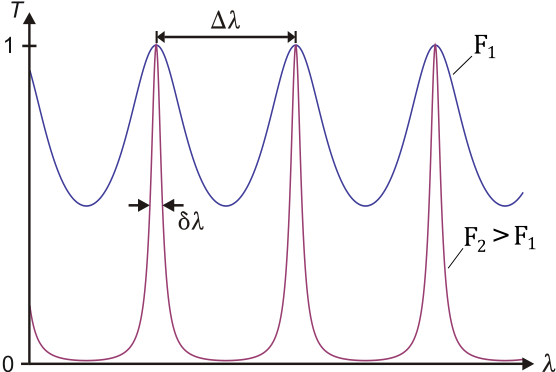
\includegraphics[width = 10cm]{Bilder/Auswertung/Finesse.png}
    \caption{Transmissionsspektrum des Fabry-Pérot-Interferometers für verschiedene Finessen }
    \label{bild:Fabry}
\end{figure}

Dabei sieht man in Abbildung \ref{bild:Fabry} schön, was unterschiedliche Finessen grafisch bedeuten.
Die Finesse 

\begin{equation}
    \mathcal{F} = \frac{\Delta \lambda}{\delta \lambda}
\end{equation}

ist das Verhältnis der Linienbreite zum Abstand der Moden. Der freie 
spektrale Bereich $\Delta \nu_{FSR}$ ergibt sich äquivalent zu Gleichung \ref{eq:FSR}. 